\sectionmark{Cytologie}

\section{Cytologie}
\label{sec:cytologie}
	\begin{enumerate}
		\item Wie funktioniert in Grundzügen ein Fluoreszenzmikroskop? Welche Unterschiede bestehen zur konventionellen Lichtmikroskopie?				
			Mit Licht in bestimmten Wellenlängen werden Stoffe
			oder auch Proteine (z.B. ``GFP'') im Objekt zum	fluoreszieren angeregt.
			So können bestimmte Strukturen sichtbar gemacht werden.
			Bei der Lichtmikroskopie wird das Objekt mit einem Spektrum des sichtbaren Lichtes
			beleuchtet.

		\item\label{tab:quest_cyt_resolution} Wie hoch ist die Auflösung eines Lichtmikroskops?
			Kennen Sie eine Formel zur Berechnung der Aufösung (vgl. Mikrobiologisches Grundpraktikum)?

		Die Auflösung eines Lichtmikroskops ist Abhängig von der Wellenlänge des Lichtes.
		Diese liegt bei grünem Licht bei 550 nm und begrenzt die die optische Auflösung.
		Die nummerische Apertur liegt bei der Verwendung von Immersionsöl bei etwa 1,3.
		Somit ist der kleinste Abstand zweier Bildpunkte bei einem 100-fach Objektiv:

		\begin{center}
		\begin{math}
			d_{0} = \dfrac{100}{1,30} = 0,3 \hspace{27mm} |\hspace{3mm} \lambda = 550nm
		\end{math}
		\end{center}

		\item Wie wirkt sich die Größe eines Organismus auf die Stoffwechselleistungen aus? Warum?
			
			Das Verhältnis von Oberfläche durch Volumen eines (kugelförmigen) Organismus,
			nimmt mit zunehmendem Radius ab.
			Dies wird mit der Oberflächenregel beschrieben, welche durch Max Rubner anhand von Säugetieren ermittelt wurde.
			Sie besagt, dass die spezifische Stoffwechselrate für (Stoffverbrauch/kg Körpergewicht)
			mit abnehmender Körpergröße ansteigt.

			Die Oberflächenregel lässt sich auch auf Mikroorganismen übertragen.
			Hier wird der Transport des Substrates über die Membran ins Cytosol zum limitierende Faktor.
			Eine Optimierung wird hier duch geringe Zellgröße und hohe Teilungsrate erreicht.
			Auch spezielle Wuchsformen wie zum Beispiel Stäbchen
			oder Fillamente und andere Zellanhängsel vergrößern die Membranfläche.

		\item Stellen Sie die Eigenschaften von Eu- und Prokaryoten einander gegenüber. Welche Eigenschaften (die Prokaryoten nicht haben) ermöglichen es Eukaryoten, große Zellen zu bilden? Warum sind dennoch einige Prokaryoten groß?

			Der Namensgebende Unterschied bezieht sich auf das Vorhandensein eines echten Zellkerns (Nucleus) bei dem Eukaryoten.
			Dieser Zellkern schließt durch eine Doppel-Lipidmembran die DNA ein
			und dient als Raum für die Transkription der DNA in mRNA.

			Bei einere prokayrotische Zelle wie in Abbildung \ref{fig:prokarya} dargestellt,
			ist somit kein Zellkern vorhanden.
			Die DNA liegt verpackt im Cytosol,
			wo auch die vollständige Proteinbiosynthese stattfindet.
			Die Verpackung der DNA geschieht jedoch im Gegensatz zu den Eukaryoten ohne Histone.
			Zusätzlich haben einige Bakterien noch ringförmige oder lineare Plasmide,
			welche als zusätzliche Träger Genmaterial dienen.
			
			\begin{figure}[ht!]
			\leavevmode
			\begin{center}
			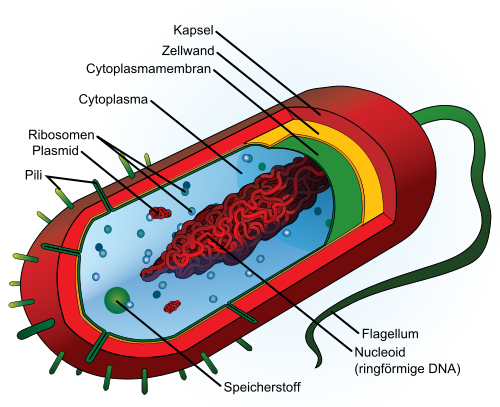
\includegraphics[scale=0.47]{./pictures/avg_prokaryote_cell_500}
			\end{center}
			\caption{\slshape{Typische prokaryotische Zelle.}}
			\label{fig:prokarya}
			\end{figure}
	
			Die Translation findet bei Prokyoten mit 70 S Ribosomen statt,
			welche frei im Cytosol vorliegen.
			Prokaryoten besitzen keine membranbegrenzten Organellen wie zum Beispiel Mitochondrien oder Vakuolen.

			\begin{figure}[ht!]
			\leavevmode
			\begin{center}
			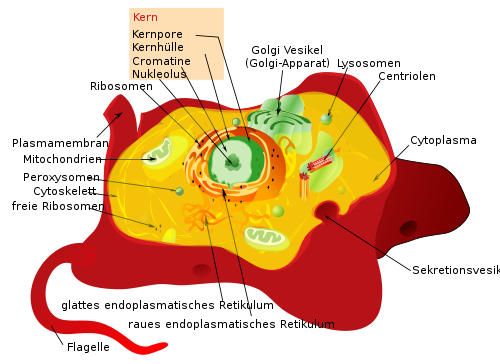
\includegraphics[scale=0.47]{./pictures/animal_cell_500}
			\end{center}
			\caption{\slshape{Tierische Zelle als Beispiel einer eukaryotischen Zelle.}}
			\label{fig:eukarya}
			\end{figure}

			Die reife mRNA wird bei Eukaryoten mit 80 S Ribosomen translatiert.
			Diese befinden sich am rauen endoplasmatischen Retikulum,
			welches bei Prokaryoten nicht vorhanden ist.
			Beispielaft für eukaryotische Zellen ist die in Abbildung \ref{fig:eukarya} dargestellte,
			tierische Zelle.

			Eukaryotische Zellen haben Transportsysteme die den Transport von Stoffen im Cytosol ermöglichen.
			Durch das Fehlen von Vakuolen in prokaryotischen Zellen sind diese in ihrer größe Beschränkt.
			Die größten Bekannten Zellen hat der \emph{Epulopiscium fishelsoni} welcher mit den Clostriedien verwandt ist.
			Seine polyploiden Zellen können über 0,5 cm groß werden,
			und maximiert so seine Oberfläche.
			
			Siehe dazu auch Frage \ref{tab:quest_cyt_resolution} in Kapitel \ref{sec:cytologie}. 

		\item Wie klein kann ein autonom lebender Prokaryot werden? Begründen Sie Ihre Abschätzung.
			
			Die kleinsten Prokaryoten mit einem Volumen von weniger als \begin{math}0,1\ \mu m^{3}\end{math} sind weit verbreitet
			in marinen Ökosystemen.
			Auch obligat symbiontische oder pathogene Bakterien können durch Reduktion ihres Zellinventares diese geringen Größen erreichen.
			Zellen mit weniger als \begin{math}0,2\ \mu m - 0,3\ \mu m\end{math} wären nicht lebensfähig,
			da zumindest Ribosomen, essentielle Metabolite sowie DNA und Proteine untergebracht werden müssen.

		\item Was sind Einheitsmembranen (unit membranes)? Wo finden sie sich in der prokaryotischen Zelle?

			Einheitsmembranen bestehen aus einer Doppelschicht von amphiphilen Fettsäuren.
			Das heisst, die Fettsäuren bestehen aus einem hydrophphilen Kopf und einem hydrophoben Schwanz.
			Bei passenden Verhältnis von Wasser zu Lipid, bildet sich spontan eine Doppelschicht der amphiphilen Fetssäuren.
			Hierbei stehen die hyprophoben Schwänze auf einander.
			Die Lipid-Doppelmembran ist etwa 5 nm dick.
		
			Die Köpfe bestehen meistens aus Phospholipiden,
			wobei am Glycerin zwei Kohlenwasserstoffketten,
			mit typischerweise zwischen 14 und 24 Kohlenstoffatomen,
			gebunden sind.
			Während eine der beiden Kohlenstoffketten meist gesättigt ist,
			hat die andere einen oder mehre \textit{cis}-Doppelbindungen.
			Dies Führt zu einer entsprechenden Anzahl von ``Knicken'' in der Kette,
			welche die Fluidität der Membran beeinflussen.
			Die Fluidität der Membran wird durch ihre Zusammensetzung bestimmt.
			So sind weitere Einflussgrößen die Temperatur und
			die Anzahl der enthaltenen Proteine.

			\begin{figure}[ht!]
			\leavevmode
			\begin{center}
			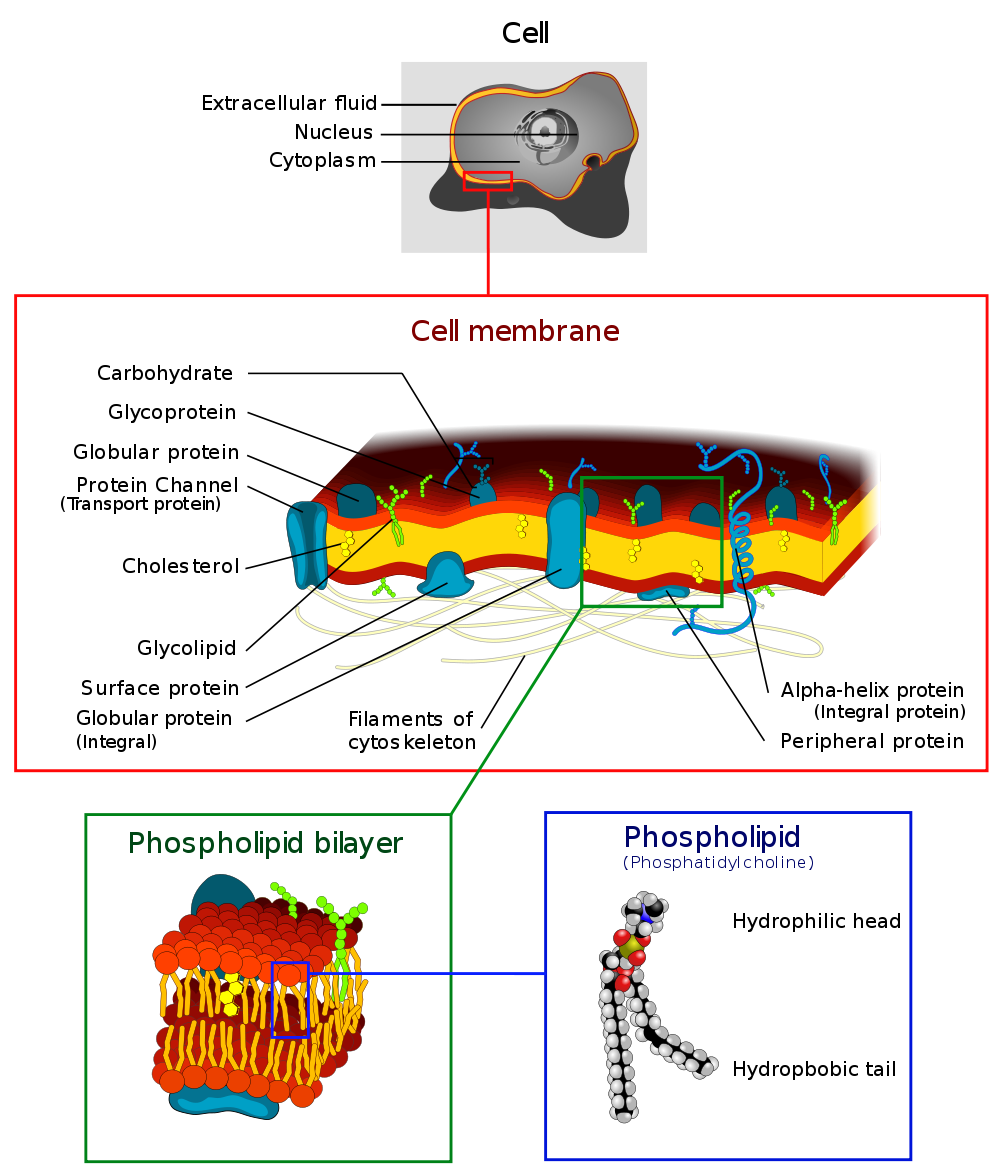
\includegraphics[scale=0.36]{./pictures/cell_membrane_diag_1000}
			\end{center}
			\caption{\slshape{Lage und Aufbau von Zellmembran.}}
			\label{fig:cellmembrane}
			\end{figure}

			Die wesentlichen Funktionen von Biomembranen sind:

			\begin{itemize}
				\item[Permeabilitätsbarriere] \hfill \\
				Selektive Barriere für den Transport ins Cytosol oder aus diesem hinnaus.
				\item[Proteinverankerung] \hfill \\
				Membranständigproteine zur gezielt Synthese von Stoffen in deffinierte Kompartimente.
				\item[Energiekonservierung] \hfill \\
				Aufbau und Verbrauch von protonenmotorischen Kräften entlang der Membran.
			\end{itemize}

		\item Wie können Membranen modifiziert werden, um sie untwrschiedlichen Umgebungstemperaturen anzupassen?
		\item Welche Proteine finden Sie typischerweise in Membranen? Welche Funktionen habe sie? Was sind Hopanoide?
		\item Stellen Sie vergleichend die unterschiedlichen Zellwand-Typen von verschiedenen Bacteria und Archaea gegenüber.
		\item Wie ist die Äußere Membran (outer membrane) von Bakterien wie z.B. \emph{Escherichia coli} gebaut?
		\item Worauf beruht die Festigkeit der Peptidoglycanstruktur? 
		\item Auf welchem Prinzip beruht die Gram-Färbung? Können Sie mit der Färbung sicher die unterschiedlichen Typen von Zellwänden unterscheiden?
	\end{enumerate}

